\documentclass[11pt]{article}
\usepackage{graphicx}
\usepackage{float}
\usepackage{amsmath}
\usepackage{amsfonts}
\usepackage[brazilian]{babel}
\usepackage[utf8]{inputenc}
\usepackage[T1]{fontenc}

\begin{document}

\title{Matemática elementar: Tipos de função - Função do primeiro grau}
\author{Erik Perillo}
\date{}
\maketitle
\begin{abstract}
Nesta etapa, começaremos a falar dos tipos de função que podemos encontrar por
aí, a começar pela mais simples delas.
\end{abstract}

\newpage

\tableofcontents

\newpage

\section{Introdução}
\paragraph{}
Na etapa anterior, começamos a falar sobre funções e a importância delas para
a matemática/cálculo. Vamos agora ir com bastante calma aprofundando nosso 
conhecimento dos tipos de funções e seus comportamentos. 
\paragraph{}
A primeira função que vamos analisar é a \emph{função do primeiro grau}. Nós
já vimos que essa função tem essa aparência no gráfico:
\begin{figure}[H]
\centering
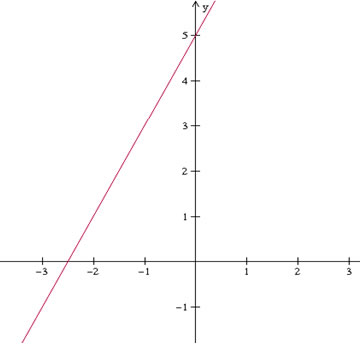
\includegraphics[width=0.5\textwidth]{imgs/funcao_afim.jpg}
\caption[9pt]{Uma típica função do primeiro grau}
\end{figure}

\section{Características}
\paragraph{}
Por que chamamos esse tipo de função de função do primeiro grau? A explicação
é que, se olharmos para a equação dessas funções, sempre temos algo do tipo:
$$f(x) = a + bx$$
Onde $a$ e $b$ são números. Por exemplo, podemos ter $f(x) = 3 + 4x$, ou 
então $f(x) = 2x$ (nesse caso, $a=0$). O que todos esses exemplos têm em 
comum é que o $x$ está sempre elevado à primeira potência neles, e é isso o 
que caracteriza uma função do primeiro grau. Uma função do tipo 
$f(x) = 3 + 4x^2$ \textbf{não} é do primeiro grau, pois o $x$ está elevado ao
quadrado nesse caso.

\subsection{Dando nome aos termos}
\paragraph{}
Já vimos que qualquer função do primeiro grau tem a forma:
$$f(x) = a + bx$$
Onde $a$, $b$ são números e $b$ não pode ser zero. 
\paragraph{}
Ao termo $a$, damos o nome de \textbf{termo constante}. Por que esse nome?
O termo $a$ não está acompanhado do $x$, então se o $x$ muda ou não, tanto
faz para ele pois ele continua a mesma coisa! Vejamos um exemplo. Seja $f$ a
função $f(x) = 3 + 2x$. Para $x=1$, temos $f(1) = 3 + 2$. Para $x=4$, temos
$f(4) = 3 + 8$. Não importa o valor de $x$, o valor 3 se mantém 3. O termo 
constante é aquele que sobra quando $x=0$. No caso do exemplo, temos 
$f(0) = 3$, que é justamente o valor do termo constante (a). Assim, ele é 
o termo que determina em que parte do eixo y a função vai cruzar quando x é
zero.
\paragraph{}
Ao termo $b$, damos o nome de \textbf{coeficiente}. Ele é o termo $b$ na
equação $f(x) = a + bx$. O coeficiente determina quão \textit{inclinada} a
reta da função é. Um coeficiente grande, deixa a reta muito inclinada. Peque
algo como, por exemplo, $f(x) = 3 + 50x$. Um coeficiente de 50 quer dizer
que a cada 1 que o x vai pra frente, o y vai 50 pra cima! 
\begin{figure}[H]
\centering
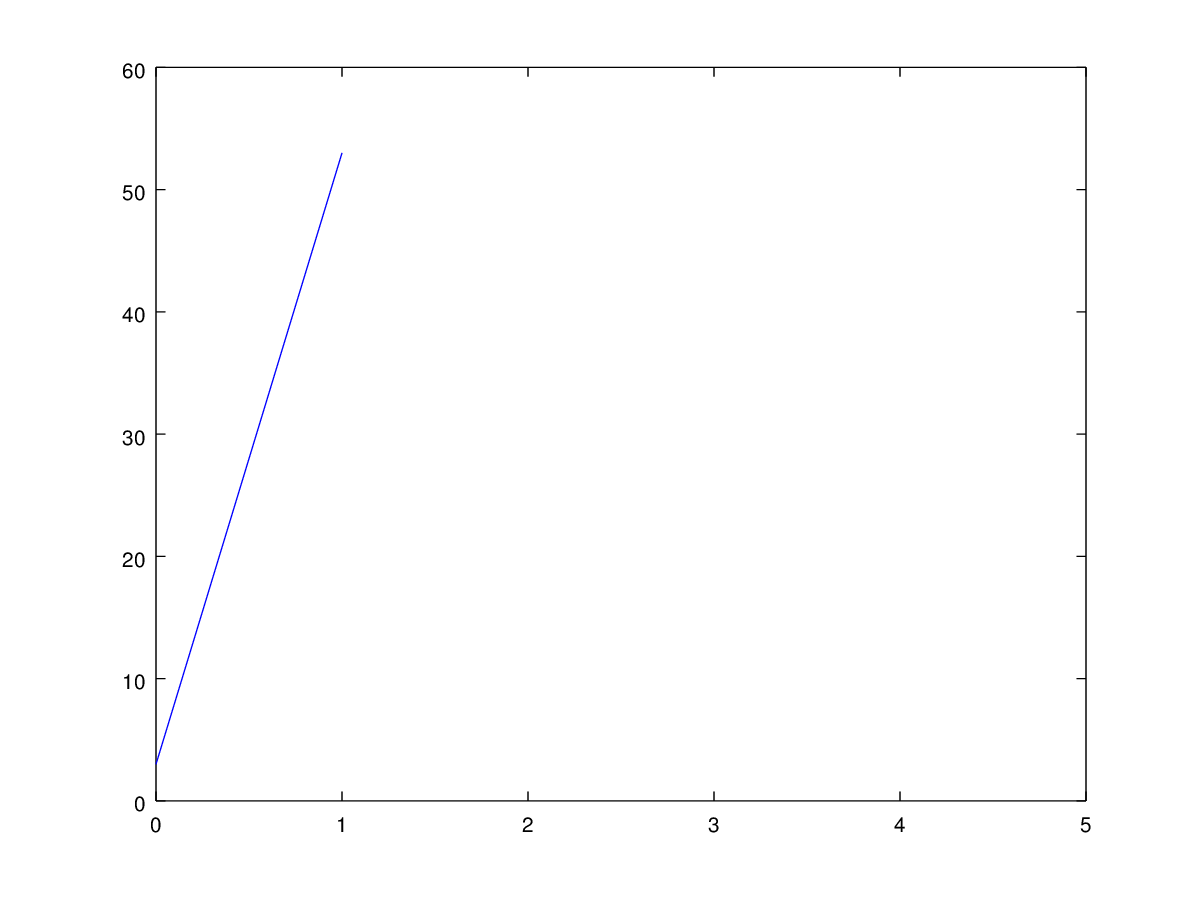
\includegraphics[width=0.7\textwidth]{imgs/reta_inclinada.png}
\caption[9pt]{Uma função com uma reta inclinada}
\end{figure}
Veja no exemplo acima como a reta fica inclinada!
\paragraph{}
Quando o coeficiente é baixo, por outro lado, ela é pouco inclinada. 
Pegando, por exemplo, $f(x) = 1 + 0.5x$, temos uma reta assim:
\begin{figure}[H]
\centering
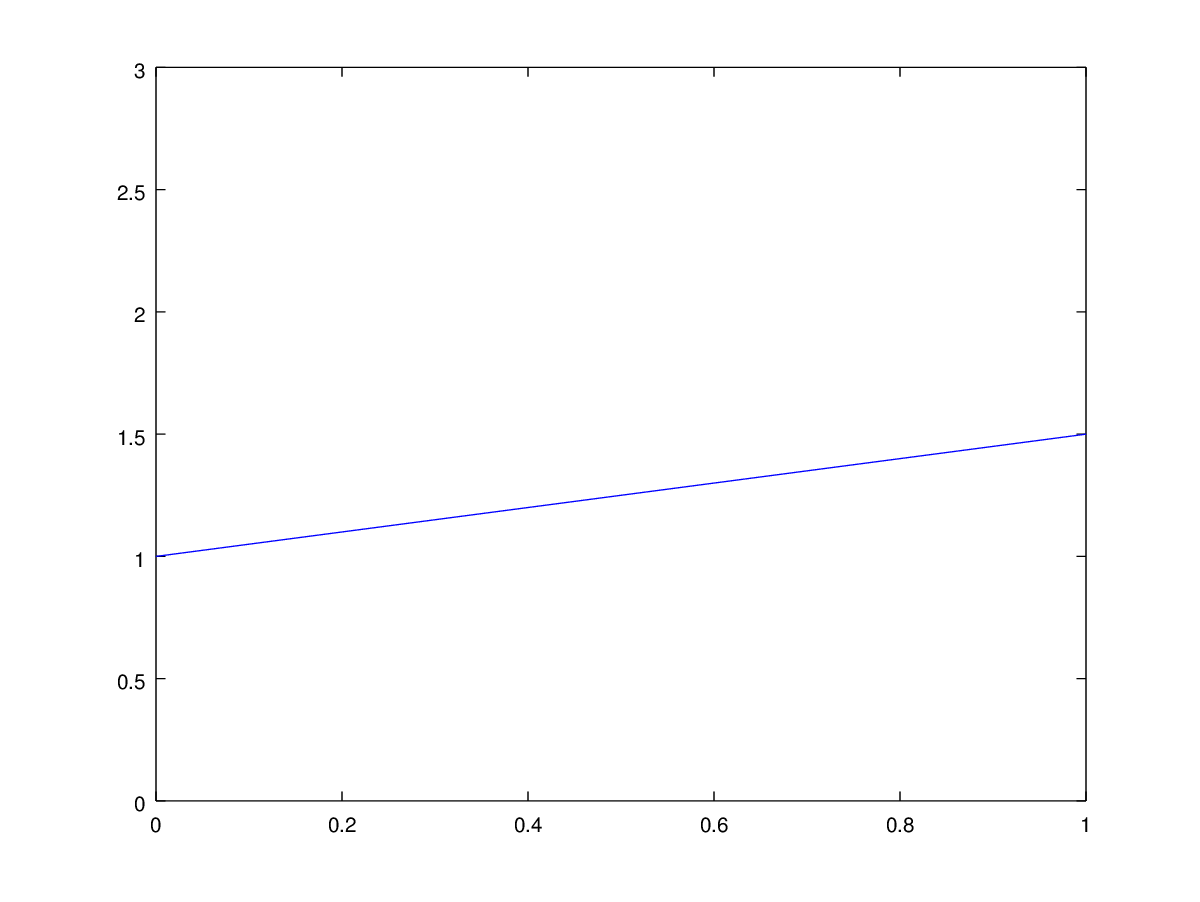
\includegraphics[width=0.7\textwidth]{imgs/reta_reta.png}
\caption[9pt]{Uma função com uma reta inclinada}
\end{figure}
Note como ela é achatada!

\section{Interseções com os eixos}
\subsection{Raiz da função}
\paragraph{}
Como já vimos antes, achar o x para que uma função $f(x)$ resulte em zero 
é achar a \emph{raiz} da função. Quando $f(x)$ resulta em zero, isso quer 
dizer que, no plano cartesiano, o ponto vai estar em $y=0$ e, assim, 
\textbf{cruzando pelo eixo x}. Para uma função do primeiro grau, é só isolar
o x:
$$f(x) = a + bx = 0$$
$$a + bx = 0 \implies bx = -a \implies x = -\frac{a}{b}$$
Assim, para \textbf{qualquer} função do primeiro grau, vamos descobrir que
a raiz dela é $-\frac{a}{b}$! Veja, por exemplo, a função $f(x) = 3 + 2x$.
Se estivermos certos, sem nem fazer conta sabemos que a raiz dela é em
$-\frac{3}{2}$. Será que é? Vamos descobrir:
$$3 + 2x = 0 \implies 2x = -3 \implies x = -\frac{3}{2}$$
E como previsto, estamos certos!
\subsection{eixo y}
\paragraph{}
Como já vimos antes, para descobrir onde no eixo y a função cruza, é só 
colocar $x=0$ na equação da função, pois quando $x=0$ a função está passando
pelo eixo y. Assim, em $f(x) = 3 + 2x$, sabemos que a função passa pelo eixo
y quando $x=0$ e então passa pelo eixo $y$ em $y = 3$.
\subsection{Visualizando o exemplo}
\paragraph{}
Visualizando o exemplo anterior $f(x) = 3 + 2x$, temos:
\begin{figure}[H]
\centering
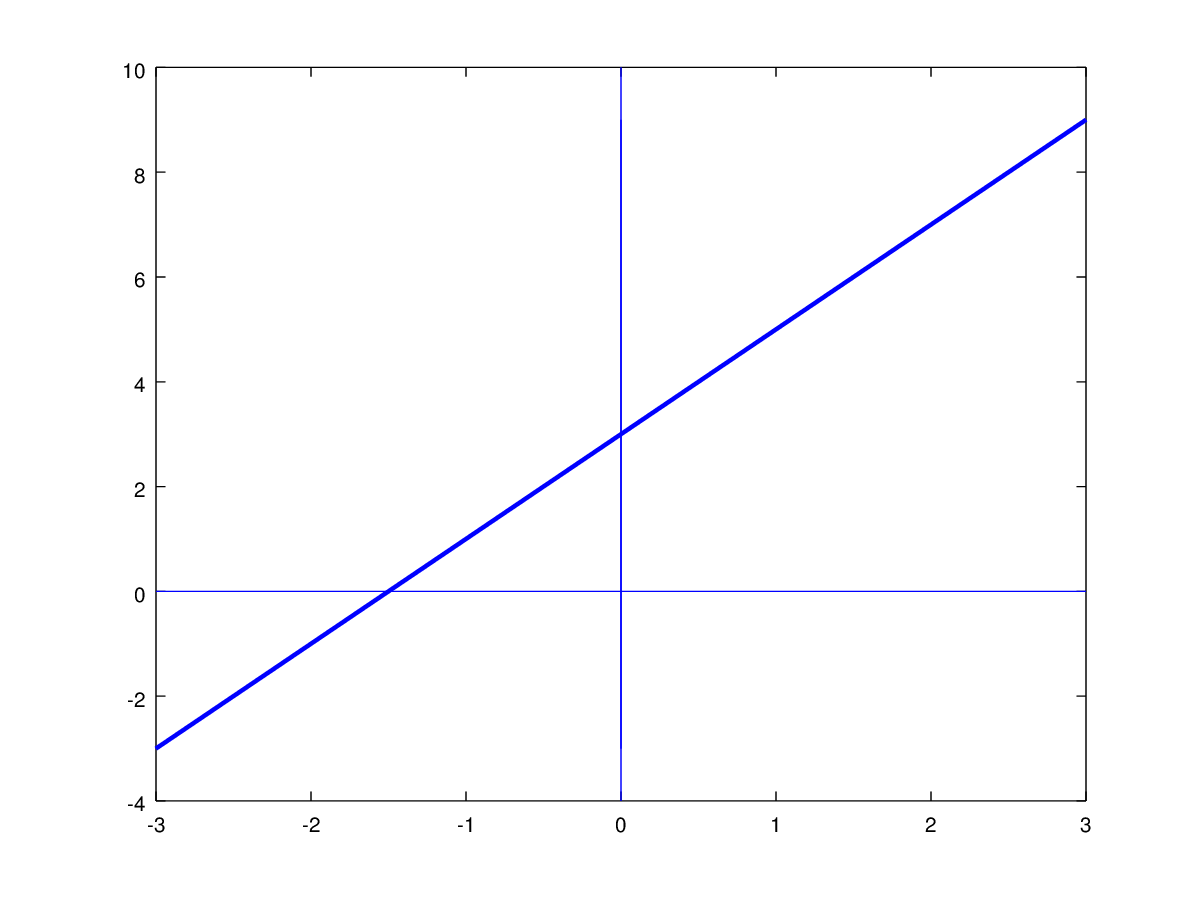
\includegraphics[width=0.9\textwidth]{imgs/raiz.png}
\caption[9pt]{Interseções}
\end{figure}
Note como passa pelo eixo x (raiz) em $x=-\frac{3}{2}$ e pelo eixo y em 
$y=3$.

\newpage

\section{Exercícios}
\begin{enumerate}
	\item Diga se as funções a seguir são do primeiro grau ou não.
		\begin{enumerate}
			\item $f(x) = 3.2 + 4.5x$
			\item $f(x) = 5$
			\item $f(x) = -5$
			\item $f(x) = -5 + 32x$
			\item $f(x) = 2x - 10$
			\item $f(x) = 3x$
			\item $f(x) = 3 + 4x^2$
			\item $f(x) = 3(1 + 2x)$
			\item $f(x) = 2 + \frac{1}{x}$
		\end{enumerate}

	\item Esboce no gráfico as funções a seguir, indicando a raiz e a 
		  interseção com os eixos x e y.
		\begin{enumerate}
			\item $f(x) = 3.2x$
			\item $f(x) = 2 + 4x$
			\item $f(x) = 1 - x$
		\end{enumerate}

	\item Diga o termo constante e o coeficiente das funções a seguir:
		\begin{enumerate}
			\item $f(x) = 3 + 2 + 4x$
			\item $f(x) = -4.2x + 5$
			\item $f(x) = 3x$
		\end{enumerate}

	\item Seja $f(x) = 2 - 4x$. Descubra o $x$ para:
		\begin{enumerate}
			\item $f(x) = 3$
			\item $f(x) = -2$
			\item $f(x) = 0$
		\end{enumerate}
\end{enumerate}

\newpage

\section{Respostas aos Exercícios}
\begin{enumerate}
	\item
		\begin{enumerate}
			\item Sim
			\item Não (coeficiente não pode ser zero)
			\item Não (coeficiente não pode ser zero)
			\item Sim
			\item Sim (tanto faz a ordem com que a função é escrita!)
			\item Sim
			\item Não (x está elevado a $2$)
			\item Sim
			\item Não (x está elevado a $-1$)
		\end{enumerate}

	\item 
		\begin{enumerate}
			\item
				\begin{figure}[H]
				\centering
				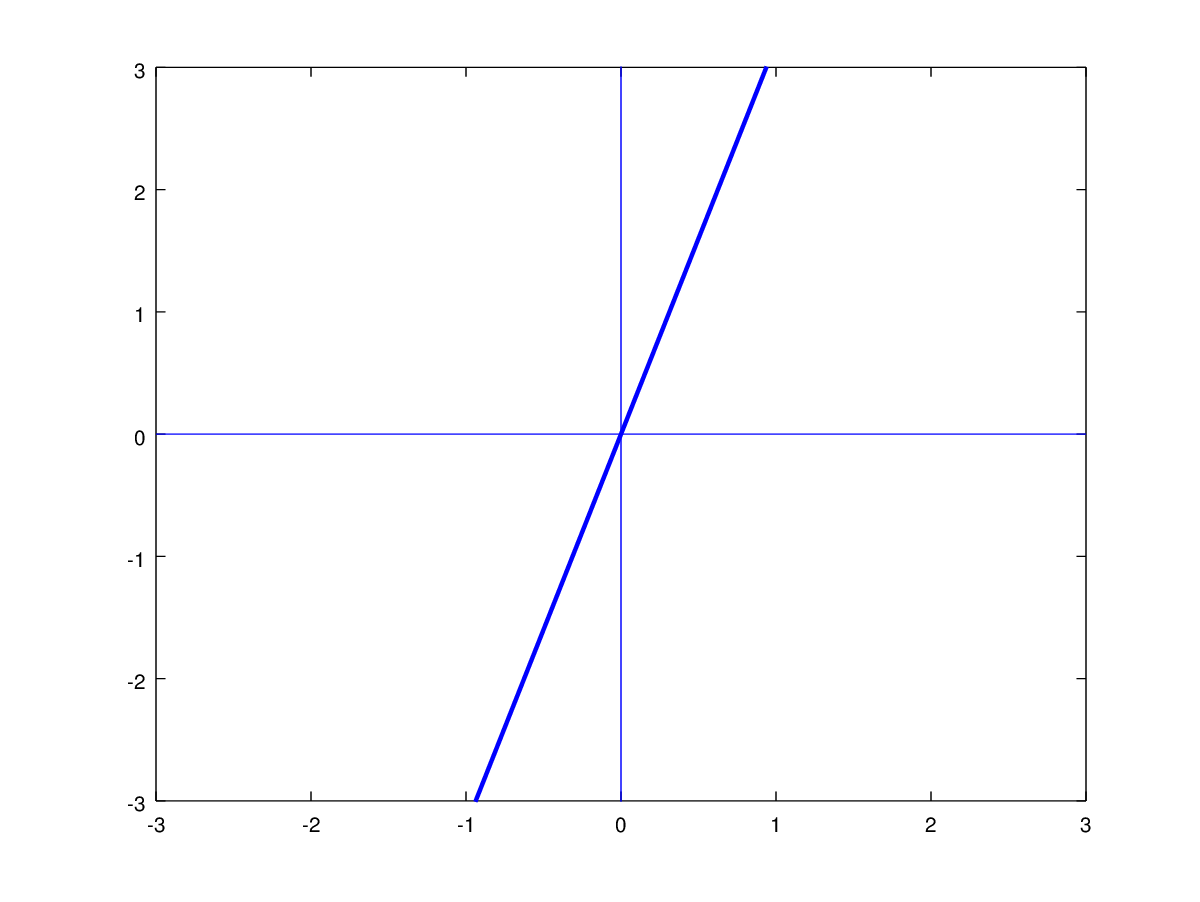
\includegraphics[width=0.6\textwidth]{imgs/explot1.png}
				\end{figure}
				Eixo x (raiz) : 0, eixo y:0
			\item
				\begin{figure}[H]
				\centering
				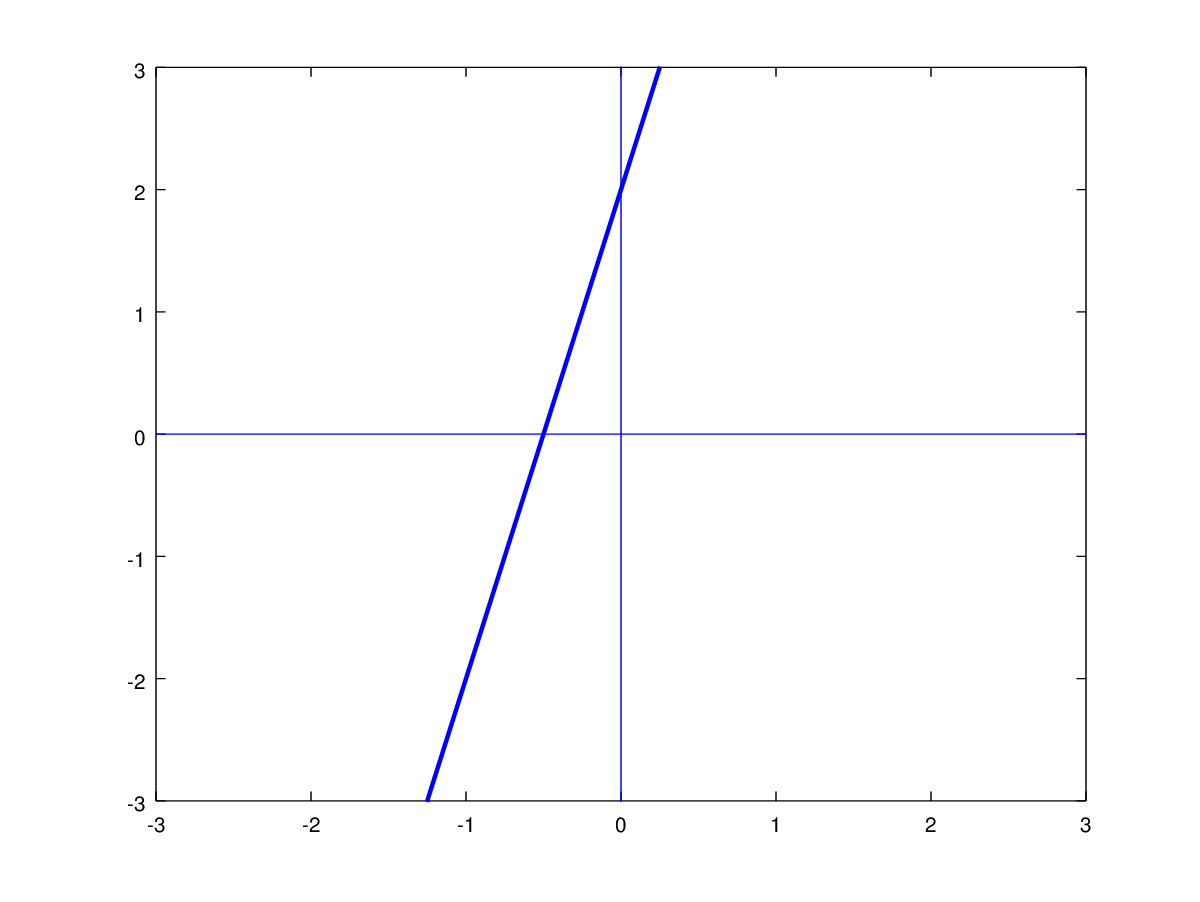
\includegraphics[width=0.6\textwidth]{imgs/explot2.png}
				\end{figure}
				Eixo x (raiz): $-0.5$, eixo y: 2
			\item $f(x) = 1 - x$
				\begin{figure}[H]
				\centering
				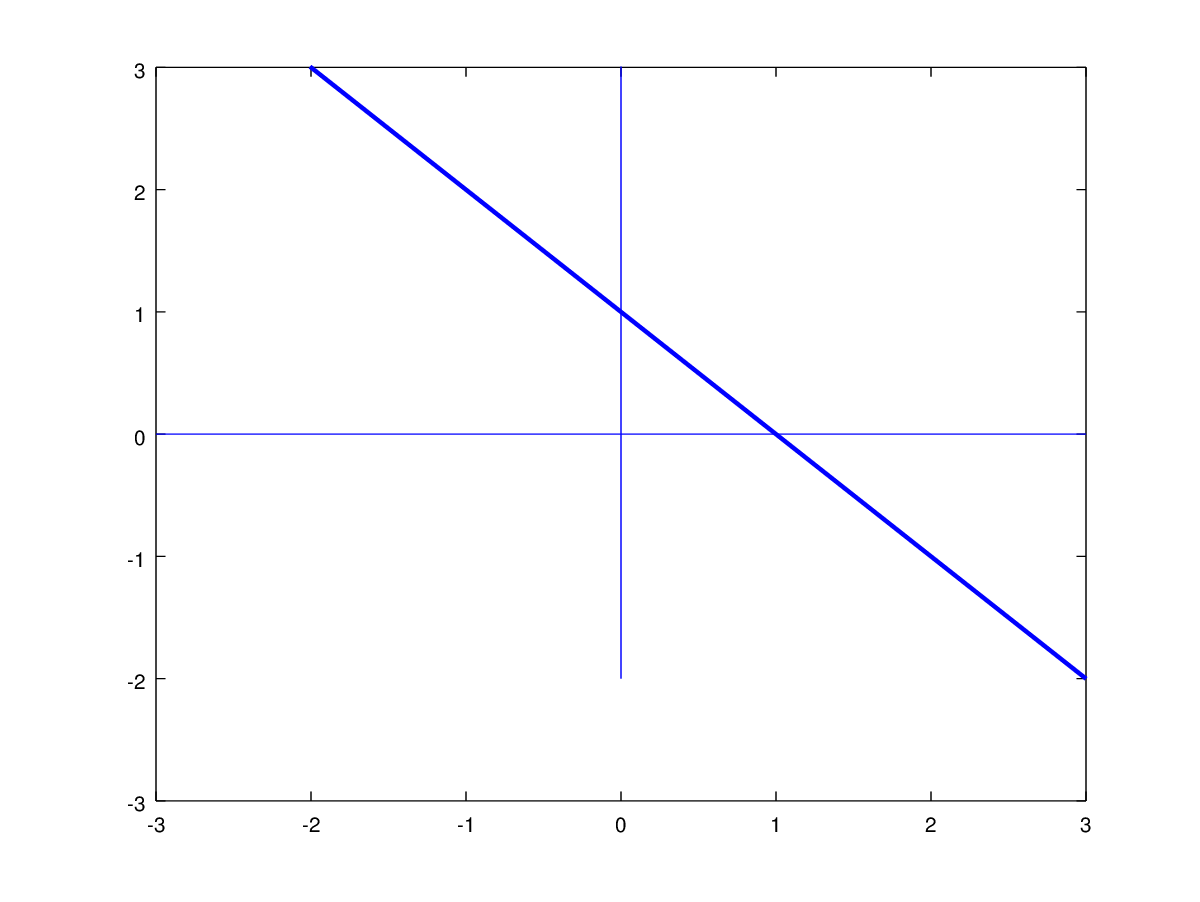
\includegraphics[width=0.6\textwidth]{imgs/explot3.png}
				\end{figure}
				Eixo x (raiz): $1$, eixo y: 1
		\end{enumerate}

	\item
		\begin{enumerate}
			\item Constante: 5, coeficiente: 4
			\item Constante: 5, coeficiente: $-4.2$
			\item Cosntante: 0, coeficiente: 3
		\end{enumerate}

	\item
		\begin{enumerate}
			\item $x = -\frac{1}{4}$
			\item $x = 1$
			\item $x = \frac{1}{2}$
		\end{enumerate}
\end{enumerate}


\end{document}
